As Figuras 1-10 apresentam a evolução do VPL da melhor solução, da pior solução e a média da população das dez execuções do Algoritmo Genético Geracional Clássico durante o Experimento 2 da Etapa 1 ($AG^{CC-2}$).

\begin{figure}[H]
\centering

\includegraphics[scale=1]{apxB/aggc/1}

\end{figure}

\begin{figure}[H]
\centering

\includegraphics[scale=1]{apxB/aggc/2}

\end{figure}

\begin{figure}[H]
\centering

\includegraphics[scale=1]{apxB/aggc/3}

\end{figure}

\begin{figure}[H]
\centering

\includegraphics[scale=1]{apxB/aggc/4}

\end{figure}

\begin{figure}[H]
\centering

\includegraphics[scale=1]{apxB/aggc/5}

\end{figure}

\begin{figure}[H]
\centering

\includegraphics[scale=1]{apxB/aggc/6}

\end{figure}

\begin{figure}[H]
\centering

\includegraphics[scale=1]{apxB/aggc/7}

\end{figure}

\begin{figure}[H]
\centering

\includegraphics[scale=1]{apxB/aggc/8}

\end{figure}

\begin{figure}[H]
\centering

\includegraphics[scale=1]{apxB/aggc/9}

\end{figure}

\begin{figure}[H]
\centering

\includegraphics[scale=1]{apxB/aggc/10}

\end{figure}

As Figuras 1-10 apresentam a evolução do VPL da melhor solução, da pior solução e a média da população das dez execuções do Algoritmo Genético de Regime Permanente Clássico durante o Experimento 2 da Etapa 1 ($AG^{RPC-2}$).

\begin{figure}[H]
\centering

\includegraphics[scale=1]{apxB/agrpc/1}

\end{figure}

\begin{figure}[H]
\centering

\includegraphics[scale=1]{apxB/agrpc/2}

\end{figure}

\begin{figure}[H]
\centering

\includegraphics[scale=1]{apxB/agrpc/3}

\end{figure}

\begin{figure}[H]
\centering

\includegraphics[scale=1]{apxB/agrpc/4}

\end{figure}

\begin{figure}[H]
\centering

\includegraphics[scale=1]{apxB/agrpc/5}

\end{figure}

\begin{figure}[H]
\centering

\includegraphics[scale=1]{apxB/agrpc/6}

\end{figure}

\begin{figure}[H]
\centering

\includegraphics[scale=1]{apxB/agrpc/7}

\end{figure}

\begin{figure}[H]
\centering

\includegraphics[scale=1]{apxB/agrpc/8}

\end{figure}


\begin{figure}[H]
\centering

\includegraphics[scale=1]{apxB/agrpc/9}

\end{figure}

\begin{figure}[H]
\centering

\includegraphics[scale=1]{apxB/agrpc/10}

\end{figure}

acabou....